\section{Oprogramowanie}
\subsection{Biblioteki peryferiów}
Na etapie planowania projektów, podjęto decyzję o samodzielnym stworzeniu bibliotek do każdego z czujników. Takie podejście, narzuciło konieczność ujednolicenia sposobu tworzenia kodu. Zdecydowano, że każda biblioteka, będzie korzystać z nakładki na funkcje HALa. Pozwoliło to wprowadzić obsługę błędów na wszystkich poziomach oprogramowania. Kod, tworzony był w sposób możliwie uniwersalny. Dzięki temu, płytka może być łatwo rozbudowana o kolejne czujniki, przy jednocześnie niewielkich zmianach w kodzie programu. Poniżej, krótko omówiono oprogramowanie każdego z czujników, oraz związane z nim biblioteki. Dla zachowania porządku, zdecydowano się rozdzielić w projekcie sterowniki dostarczane przez ST, pliki nagłówkowe oraz stworzone biblioteki. Zastosowanie opisanego w rozdziale \ref{cha:introduction} makefile, pozwoliło w łatwy sposób zdefiniować ścieżki dla kompilatora.
\newline
\textbf{BMP280}
\newline
Pierwszy z czujników, jest czujnikiem komunikującym się z mikroprocesorem z wykorzystaniem SPI (Serial Peripheral Interface). Pozwala on na wykonywanie pomiarów temperatury oraz ciśnienia. Stworzona biblioteka \textit{,,spi.c''} pozwala w łatwy sposób zainicjalizować peryferium w zdefiniowany sposób, odpowiedni dla stworzonej płytki. Osobna funkcja inicjalizująca piny SS (Slave Select) umożliwia szybkie dodanie kolejnych czujników działających z użyciem SPI. Wymaga to jedynie zainicjalizowania pinu. Dwie kolejne funkcje, odpowiadają za kolejno wysyłanie i odczytywanie danych przy użyciu SPI. Interesującym kierunkiem rozbudowy biblioteki, byłaby możliwość rejestracji pinów SS, co zdjęłoby z użytkownika konieczność samodzielnej kontroli nad używanym interfejsem oraz pinami. W przypadku tej wersji płytki, nie było to jednak konieczne. Biblioteka \textit{,,bmp280.c''} korzystająca z \textit{,,spi.c''}, odpowiada za podstawową obsługę czujnika BMP280. Poza podstawowymi możliwościami konfiguracji zgodnie z dokumentacją producenta, wykonuje wszelkie obliczenia, zdejmując z użytkownika konieczność przeliczenia danych z rejestrów.
\newline
\newline
\textbf{STS3x-DIS}
\newline
Kolejny z czujników to czujnik temperatury. Od poprzednika, różni się większą złożonością i lepszą precyzją. Do komunikacji, wykorzystuje magistralę I$^2$C. Stworzona do jego obsługi biblioteka, pozwala zmieniać jego konfigurację przy użyciu czytelnych stałych. Zapewnia nie tylko obsługę rejestrów czujnika, ale również kontrolę CRC otrzymywanych danych. Dzięki temu, użytkownik może być pewien otrzymywanych wartości.
\newline
\newline
\textbf{MQ-2}
\newline
Ostatni z czujników, to analogowy czujnik gazów. Stworzona do obsługi konwertera A/D inicjalizuje wybrane ADC mikoprocesora oraz konkretny kanał, według wartości odpowiednich dla stworzonej płytki. Posiada również funkcję pobrania próbki wybranego konwertera. Sama biblioteka obsługująca MQ-2, poza inicjalizacją i kalibracją sensora, pozwala użytkownikowi na pobranie przetworzonych lub surowych danych z czujnika, dla wybranego gazu. Dodatkową funkcją, jest możliwość ustawienia alarmu dla wybranego gazu, na zdefiniowany przez użytkownika próg. Przekroczenie wybranej wartości wyzwoli alarm oraz wysteruje pin INT standardu mikroBUS\texttrademark. Aby umożliwić swobodne tworzenie funkcji przerwań czasowych w dowolnej ilości, stworzona została biblioteka \textit{,,timers.c''}. Przy użyciu jednokierunkowej, dynamicznej listy stuktur oraz mechanizmu SysTick (przerwania wyzwalanego co 1ms) użytkownik może dodawać własne funkcje o predefiniowanym typie, a następnie wywołać je po upływie określonego czasu. Dodatkowa flaga, pozwala włączyć okresowe wyzwalanie danej funkcji. Zaletą tego podejścia jest przede wszystkim ,,nieograniczona'' liczba liczników, jednak niepoprawne wykorzystanie biblioteki (np. funkcje o długim czasie wykonywania), może prowadzić do utraty precyzji liczników.
\newline
\newline
\textbf{CP2102}
\newline
Na potrzeby obsługi konwertera UART-USB, służącego do debugu kodu, stworzona została również prosta biblioteka do obsługi UARTu. Zawiera ona konfigurację peryferium oraz funkcję działającą jak printf, która zamiast na wyjście standardowe, kieruje dane na konkretny UART. W podobny sposób działa biblioteka obsługująca UART do komunikacji użytkownika z mikroprocesorem, wspomniana w podrozdziale \ref{sub:api}. Zostały one rozdzielone ze względu na zachowanie czystości w kodzie.
\subsection{API}
\label{sub:api}
Najważniejszym elementem projektu, spinającym wszystko w jedną całość, jest stworzone API (ang. Application Programming Interface). Pozwala ono użytkownikowi na komunikację z czujikami, przy użyciu interfejsu UART. Zdecydowano, że dla uproszczenia komunikacji, układ będzie zachowywać się podobnie do dostępnych na rynków modemów, wykorzystując komendy z przedrostkiem \textit{,,AT+''}. Diagram \ref{img:api_diagram} przedstawia schemat działania API. Zostało ono zrealizowane przy użyciu stałych tablic struktur, zawierających komendę oraz związany z nią callback, czyli wywołanie odpowiedniej funkcji bibliotek sensora. Dla ułatwienia obsługi oraz lepszej czytelności kodu, każdy z czujników posiada własną tablicę wywołań. Tym samym, działanie całego API, to tak naprawdę jedna pętla, wywoływana po wykryciu przez UART komendy \textit{,,AT+''}. Wyszukuje ona komendę na odpowiedniej liście, a następnie wywołuje związaną z nią funkcję. Takie podejście, pozwala w bardzo łatwy sposób rozbudowywać kod w przypadku chęci wykorzystania kolejnych czujników. Jedyne wymagane zmiany, to dodanie kolejnej listy zawierającej komendy oraz powiązane callbacki. Zgodnie z diagramem \ref{img:api_diagram}, w przypadku nierozpoznania komendy \textit{AT} układ zwraca użytkownikowi informację \textit{UNKNOWN} (ang. nieznany). \textbf{Kolejne komendy, rozpoznawane są przez znak kończący linię \textbackslash r}. W przypadku nierozpoznanych danych, przesłanych do mikroprocesora, zwrócona zostanie informacja \textit{ERROR} (ang. błąd).

\begin{figure}[H]
    \centering
    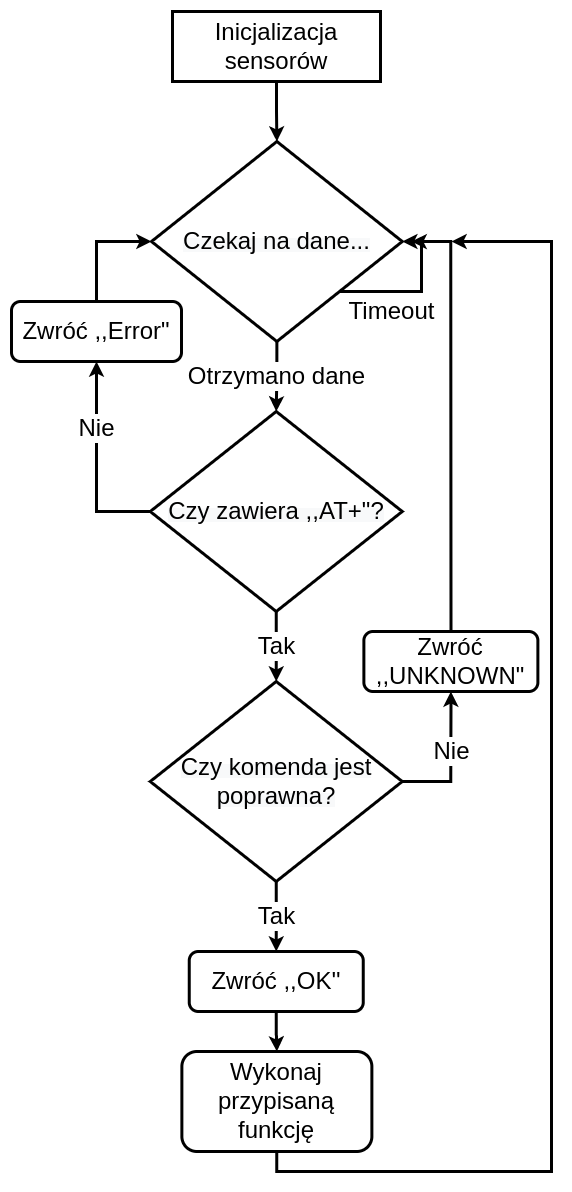
\includegraphics[width=\textwidth, height=\textheight, keepaspectratio]{Graphics/API_Sensors.png}
    \caption{Diagram działania API}
    \label{img:api_diagram}
\end{figure}

\subsection{Lista dostępnych funkcji}
\textbf{W przypadku poprawnego użycia funkcji, moduł zwróci komendę ,,OK''. Niepoprawna komenda dla danego sensora, skutkuje błędem ,,UNKNOWN'', a zbiór złych danych powoduje ,,ERROR''. Dodatkowo, w przypadku komend zawierających parametry, poza powyższymi, układ zwróci ,,0'' w przypadku poprawnego odczytania parametrów lub ,,1'' w przypadku błędu.}\newline\newline

\textbf{Ogólne}\newline
   ,,AT+BMP\textbackslash r'' - Wybiera czujnik BMP280\newline
   ,,AT+STS\textbackslash r'' - Wybiera czujnik STS3x-DIS\newline
   ,,AT+MQ\textbackslash r'' - Wybiera czujnik MQ-2\newline
   ,,AT+BACK\textbackslash r'' - Powrót do menu wyboru czujników\newline

\textbf{BMP280}\newline
   ,,AT+GETTEMP\textbackslash r'' - Odczytuje próbkę temperatury\newline
   ,,AT+GETPRESSURE\textbackslash r'' - Odczytuje próbkę ciśnienia\newline
   ,,AT+SETCONFIG,\lbrack temp\rbrack,\lbrack pressure\rbrack,\lbrack standby\rbrack,\lbrack mode\rbrack\textbackslash r'' - Ustawia konfigurację według parametrów z dokumentacji producenta: \lbrack temp\rbrack - temperature\textunderscore sampling, \lbrack pressure\rbrack - pressure\textunderscore sampling, \lbrack standby\rbrack - standby\textunderscore period, \lbrack mode\rbrack - running\textunderscore mode. Eg. \textit{AT+SETCONFIG,128,16,0,3\textbackslash r}\newline
   ,,AT+WAITRDY\textbackslash r'' - Czeka na flagę RDY rejetru statusowego. Timeout = 20s.\newline
   ,,AT+SREST\textbackslash r'' - Programowy reset czujnika\newline
   ,,AT+BACK\textbackslash r'' - Powrót do menu wyboru czujników\newline

\textbf{MQ-2}\newline
   ,,AT+GESAMPLE\textbackslash r'' - Odczytuje surową wartość ADC.\newline
   ,,AT+GETLPG\textbackslash r'' - Odczytuje przeliczone stężenie LPG.\newline
   ,,AT+GETCO\textbackslash r'' - Odczytuje przeliczone stężenie CO.\newline
   ,,AT+GETSMOKE\textbackslash r'' - Odczytuje przeliczone stężenie dymu.\newline
   ,,AT+SETTRACKING,\lbrack timeout\rbrack,\lbrack gas\rbrack,\lbrack threshold\rbrack\textbackslash r'' - Ustawia śledzenie stężenia wybranego gazu. Po wyzwoleniu alarmu, pin INT ustawiany jest w stan niski. Przerwanie czyszczone jest w momencie odczytu dowolnych danych. \lbrack timeout\rbrack - Okres między próbkami, \lbrack gas\rbrack - wybrany gaz (0-LPG, 1-CO, 2-SMOKE), \lbrack threshold\rbrack - Wartość progowa alarmu.\newline
   ,,AT+STOPTRACKING\textbackslash r'' - Przerywa śledzenie gazu. Czyści przerwanie, jeśli wystąpiło. \newline
   ,,AT+BACK\textbackslash r'' - Powrót do menu wyboru czujników\newline

\textbf{STS3x-DIS}\newline
   ,,AT+GETDATA\textbackslash r'' - Odczytuje próbkę temperatury\newline
   ,,AT+SETREPL\textbackslash r'' - Ustawia dokładność na niską \newline
   ,,AT+SETREPM\textbackslash r'' - Ustawia dokładność na średnią\newline
   ,,AT+SETREPH\textbackslash r'' - Ustawia dokładność na wysoką\newline
   ,,AT+SETHEATON\textbackslash r'' - Włącza wewnętrzną grzałkę\newline
   ,,AT+SETHEATOFF\textbackslash r'' - Wyłącza wewnętrzną grzałkę\newline
   ,,AT+SRESET\textbackslash r'' - Programowy reset czujnika\newline
   ,,AT+BACK\textbackslash r'' - Powrót do menu wyboru czujników\newline

\subsection{System kontroli wersji}
Jak wspomniano we wstępie, podczas projektu korzystano z systemu kontroli wersji Git, na platformie Github. Na jego potrzeby, stworzono dwa repozytoria:\newline
\textbf{Software}\newline
\url{https://github.com/RadoslawSajdak/Sensors_in_embedded_systems_software}\newline
\textbf{PCB}\newline
\url{https://github.com/RadoslawSajdak/Sensors_in_embedded_systems_PCB}\newline
\newline
W przypadku pierwszego z nich:
\begin{itemize}
    \item Wykonano 16 pull requestów
    \item Stworzono 22 gałęzie
    \item Wykonano 100 commitów
    \item Napisano 2264 linii kodu + pliki konfiguracyjne
\end{itemize}
Skorzystanie z platformy Github pozwoliło przede wszystkim na pełną kontrolę, nad kodem opisanym przez powyższe liczby. W trakcie wykonywania projektu, był on nieustannie sprawdzany pod kątem poprawności składni, dobrych praktyk w tworzeniu kodu, a także testowany manualnie. Możliwość przejrzystej dyskusji, pozwoliła wszystkim członkom zespołu nauczyć się wielu nowych technik, a także spojrzeć na kod z cudzej perspektywy. Takie podejście, zdecydowanie jest dobrą praktyką, pozwalającą uniknąć wielu godzin poszukiwania błędów. W swojej książce \textit{Pragmatyczny programista. Od czeladnika do mistrza.} Andrew Hunt oraz David Thomas piszą: ,,Zawsze należy stosować system kontroli kodu źródłowego. Zawsze. Nawet jeśli stanowimy jednoosobowy zespół i jeśli cały projekt zajmuje zaledwie tydzień. Kontroli kodu źródłowego, powinno podlegać dosłownie wszystko''\cite{pragmatic}.